\section{Ergebnisse}

\subsection{Webansicht}
Die Standardansicht der Webseite sieht wie folgt aus. 
\begin{figure}[h]
\centering
	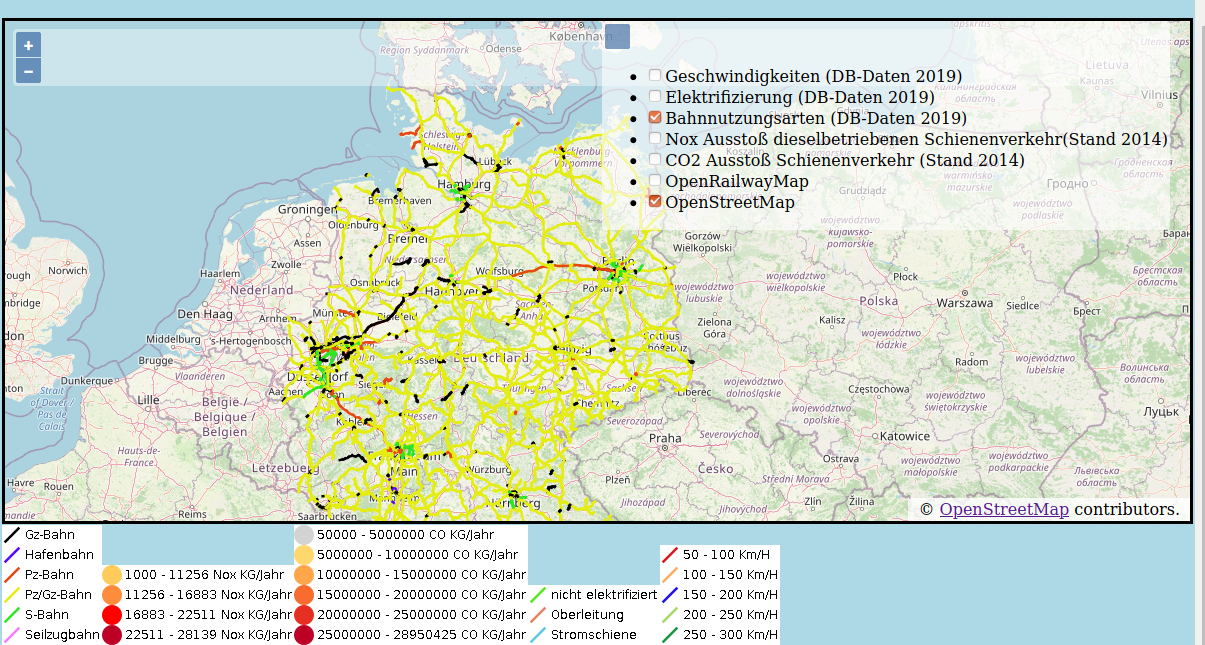
\includegraphics[width=0.9\textwidth]{images/defaultview.png}
	\caption{Default view from the webapplikation}
\end{figure}
Zentral wird die Karte mit der aktuell ausgewählten Zoomstufe angezeigt. Die Zoomstufe lässt sich über die Buttons oben links ändern. Auf der rechten Seite ist der LayerSwitcher zu sehen, dieser ermöglicht es alle Layer in verschiedenen Kombinationen anzuzeigen. Am Unteren Rand der Karte sind die Legenden der Layer zu erkennen.
\pagebreak
\subsection{Datenanalyse}
Anhand der Visualisierung sind einige Auffälligkeiten zu erkennen.
In Norddeutschland auf der Zugstrecke auf die Insel Sylt gibt es einen der höchsten Ausstoß von Stickoxide durch den Dieselverkehr in Deutschland. In Norddeutschland sind ungefähr ein drittel der Bahninfrastruktur elektrifiziert.\cite{marschbahn} Und da regelmäßig Dieselloks auf die Insel Sylt fahren um den Tourismus zu unterstützen, ist dies eine vielbefahrene Strecke. Diese Strecke führt über den Hindenburgdamm eingleisig nach Sylt, dies bedeutet es kann auch häufig zum Stau kommen, welcher ebenfalls für die erhöhte Umweltbelastung spricht. \cite{marschbahn}
\begin{figure}[h]
\centering
	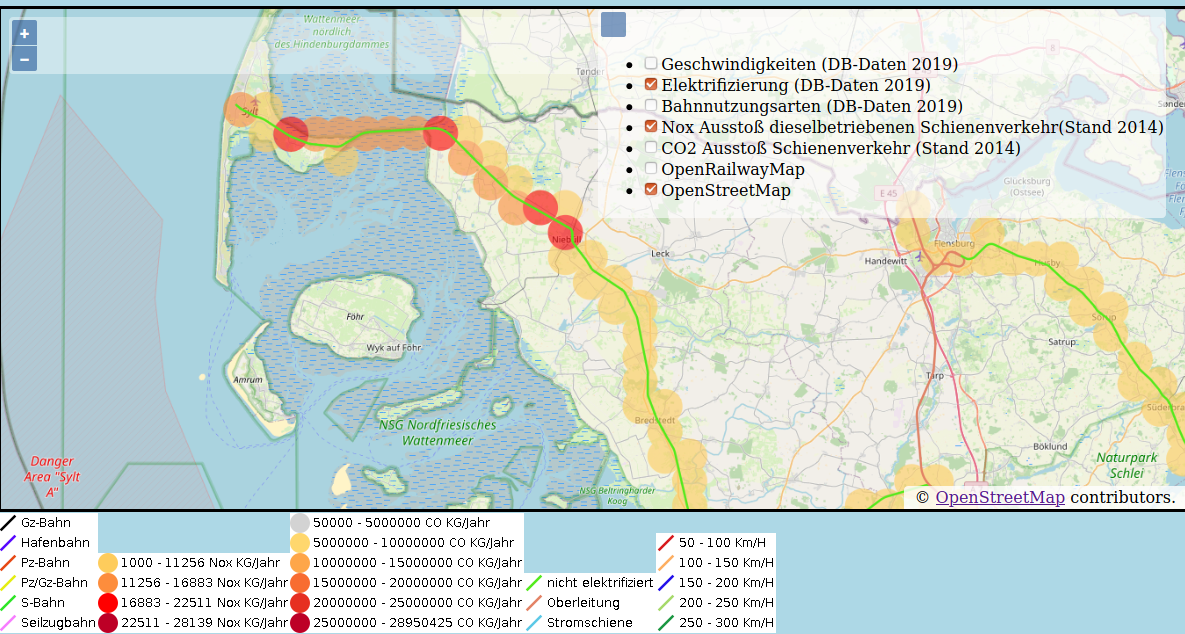
\includegraphics[width=0.7\textwidth]{images/Analyse1.png}
	\caption{Stickoxid Ausstoß in Norddeutschland}
\end{figure}
Der Ausstoß von CO2 ist nur den Ballungsgebieten deutlich erhöht. Die höchsten gemesenen Werte Gemessener Ausstoß vom Schienenverkehr in dichtbesiedelten Städten höher.
\begin{figure}[h]
\centering
	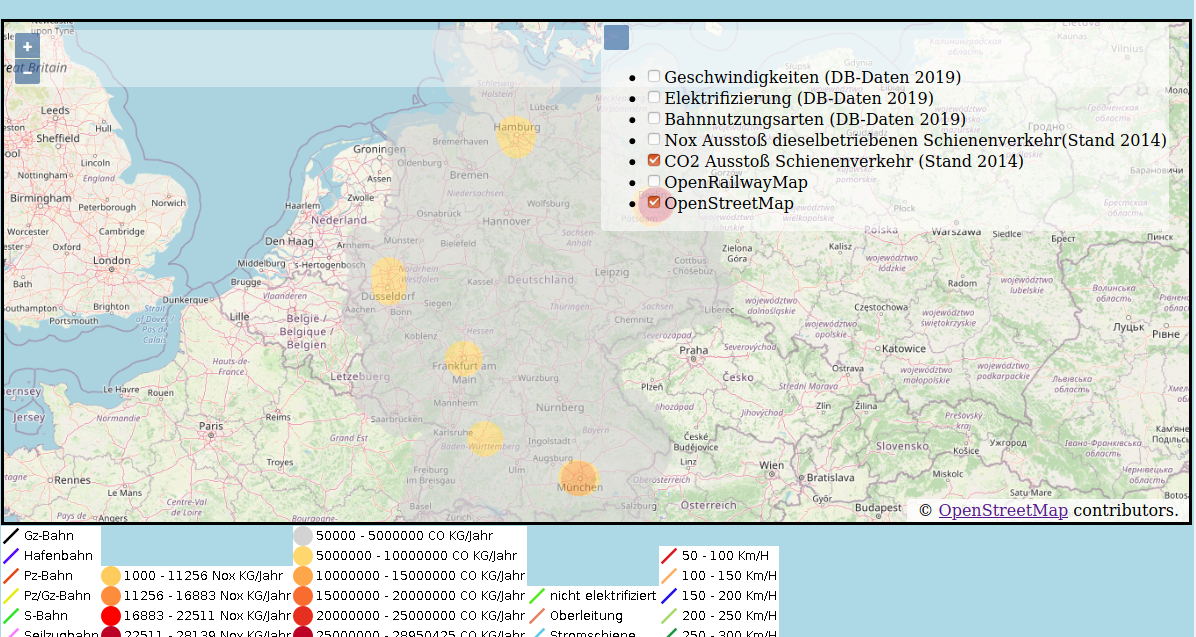
\includegraphics[width=0.7\textwidth]{images/Analyse3.png}
	\caption{CO2 Ausstoß der Deutschen Bahn}
\end{figure}
Ein weiterer Aspekt der im aktuellen Deutschenschienennetz auffällt, ist das sehr wenig Strecken auf Höchstgeschwindigkeit ausgelegt sind. Was bedeutet, dass ICE vorallem der neueren Generationen nur auf kurzen Streckenabschnitten die Gelegenheit haben ihre maximal Geschwindigkeit zu erreichen.
\begin{figure}[h]
\centering
	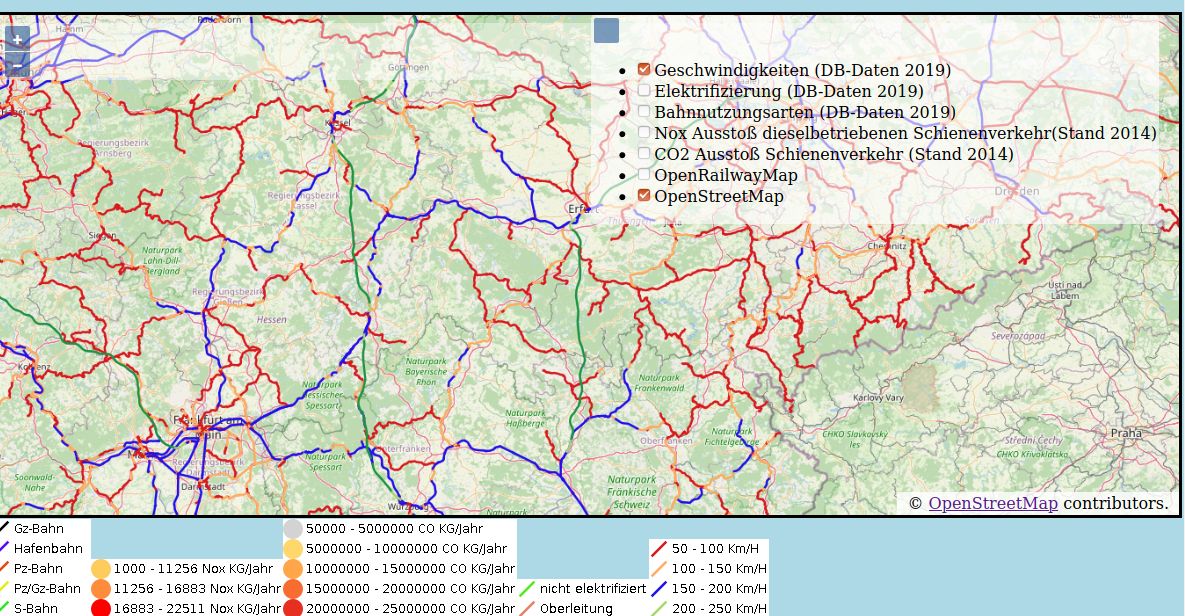
\includegraphics[width=0.7\textwidth]{images/Analyse2.png}
	\caption{Ausschnitt der Höchstgeschwindigkeit des Streckennetztes}
\end{figure}
Die Strecken ab Mitteldeutschland bis Süddeutschland sind teilweise auf bis zu 300 Km/h ausgerichtet. Von Westdeutschland nach Ostdeutschland gibt es keine Einzige Strecke die für Höchstgeschwindigkeit eines ICE ausgerichtet ist.
Die meisten Streckenabschnitte in Deutschland bieten eine Höchstgeschwindigkeit von 150 - 200 Km/h.
